\newpage
\section{IMPACTO SOCIAL, ECONÓMICO Y MEDIOAMBIENTAL} \label{impacto}

A continuación, se detallan las contribuciones al desarrollo social, económico y medioambiental de la temática trabajada en el proyecto: los \acrlongpl{smr} y la simulación para la educación y formación nuclear. Para ello, se toman como referencia los Objetivos de Desarrollo Sostenible (ODS) y se explica el modo en el que se potencian algunos de ellos:

\begin{itemize}
    \item \textbf{Objetivo 1 - Fin de la pobreza:} La meta 4 de este ODS consiste en \textit{``garantizar que todos los hombres y mujeres, en particular los pobres y los más vulnerables, tengan los mismos derechos a los recursos económicos, así como acceso a los servicios básicos, la propiedad y el control de las tierras y otros bienes, la herencia, los recursos naturales, las nuevas tecnologías y los servicios económicos''} (\cite{ODS}).
    
    Tal y como se explica en el punto \ref{zonas_remotas} \textit{Abastecimiento de zonas remotas}, la pobreza energética es una realidad en muchos países del mundo y hoy en día existen regiones muy extensas en las que se carece completamente de acceso a la electricidad, o regiones en los que este acceso es muy limitado e inestable. Es cierto que, para países subdesarrollados o en vías de desarrollo, la construcción de grandes centrales nucleares puede resultar inviable, pero el empleo de \acrshortpl{smr} se está planteando seriamente como una solución eficiente y competitiva, tal y como se se observa en la figura \ref{fig:africa_nuclear_support} del apartado \ref{zonas_remotas}. La flexibilidad en el despliegue de estos pequeños reactores modulares ---en apoyo a las fuentes de energía renovables---, permite tanto el abastecimiento independiente de zonas remotas que no están conectadas a una red eléctrica, como el desarrollo de un sistema eléctrico más interconectado para cubrir la demanda eléctrica total de regiones enteras.

    \item \textbf{Objetivo 4 - Educación de calidad:} La meta 4 de este ODS se propone \textit{``aumentar considerablemente el número de jóvenes y adultos que tienen las competencias necesarias, en particular técnicas y profesionales, para acceder al empleo, al trabajo decente y al emprendimiento''} (\cite{ODS}).
    
    Como se ha explicado en el apartado \ref{simuladores}, el empleo de simuladores en el ámbito nuclear es una herramienta muy efectiva para la adquisición de los conocimientos, técnicas y habilidades imprescindibles para la comprensión de los principios fundamentales de la tecnología nuclear y para la óptima operación de las centrales nucleares. La experiencia ha demostrado que para la profunda comprensión de una tecnología tan compleja y avanzada como la nuclear, no es suficiente con explicaciones teóricas, sino que se requiere también de una experimentación práctica.  De esta manera, el empleo de los simuladores actualmente disponibles y el desarrollo de nuevos, supone una aportación importante para la competente formación tanto en el ámbito académico como profesional del sector nuclear.

    \item \textbf{Objetivo 6 - Agua limpia y saneamiento:} La meta 6 de este ODS se plantea \textit{``ampliar la cooperación internacional y el apoyo prestado a los países en desarrollo para la creación de capacidad en actividades y programas relativos al agua y al saneamiento, como los de captación de agua, desalinización, uso eficiente de los recursos hídricos, tratamiento de aguas residuales, reciclado y tecnologías de reutilización''} (\cite{ODS}).
    
    Una de las aplicaciones ya empleada en algunas centrales nucleares actuales y potenciada especialmente en el diseño de los \acrlongpl{smr}, es la \textbf{desalación}. Tal y como se detalla en el punto \ref{cogeneracion}, numerosos países han apostado y quieren apostar por dar a los \acrshortpl{smr} el uso adicional de suministrar la energía eléctrica y térmica necesaria para el funcionamiento de sus desaladoras, contribuyendo así a mejorar el abastecimiento de agua limpia.

    \item \textbf{Objetivo 7 - Energía asequible y no contaminante:} La meta 1 de este ODS se propone \textit{``garantizar el acceso universal a servicios energéticos asequibles, fiables y modernos''}, al mismo tiempo que la meta 3 del mismo busca \textit{``duplicar la tasa mundial de mejora de la eficiencia energética''} (\cite{ODS}).
    
    Como se ha comentado en la \textit{Introducción} (apartado \ref{sec:introduccion}) del presente proyecto, la energía nuclear ayuda a los países a satisfacer la creciente demanda de energía, al tiempo que mejora la seguridad energética, reduce los efectos ambientales y en la salud derivados de la producción de energía poco responsable, y mitiga el cambio climático. En concreto, como ya se ha mencionado en múltiples ocasiones, los pequeños reactores modulares tienen la gran ventaja de ser una tecnología nuclear más asequible, tal y como se específica en el apartado \ref{economia} de \textit{Costes y competitividad}.

    \item \textbf{Objetivos 8 - Trabajo decente y crecimiento económico y 9 - Industria, innovación e infraestructura} Por una parte, se busca \textit{``lograr niveles más elevados de productividad económica mediante la diversificación, la modernización tecnológica y la innovación''}. Por otra parte, se propone \textit{``promover políticas orientadas al desarrollo que apoyen las actividades productivas, la creación de puestos de trabajo decentes, el emprendimiento, la creatividad y la innovación, y fomentar la formalización y el crecimiento de las microempresas y las pequeñas y medianas empresas''} (\cite{ODS}).
    
    En primer lugar, con la realización de este proyecto, se ha podido comprobar que los \acrlongpl{smr} son una tecnología avanzada, moderna y viable. Además, su desarrollo está potenciando la creación de numerosas empresas especializadas ---que proponen y diseñan conceptos de \acrshortpl{smr} de todo tipo---, y el surgimiento de asociaciones e infraestructuras para su implementación a corto plazo.

    \item \textbf{Objetivo 12 - Producción y consumo responsable:} La meta 1 de este ODS busca \textit{``lograr la gestión sostenible y el uso eficiente de los recursos naturales''}, al mismo tiempo que la meta 5 propone \textit{``reducir considerablemente la generación de desechos mediante actividades de prevención, reducción, reciclado y reutilización''} (\cite{ODS}).
    
    Las centrales nucleares ---y, de modo particular, los reactores avanzados--- se caracterizan por un empleo eficiente del combustible, de forma que una pequeña cantidad de recurso mineral proporciona una gran cantidad de energía. Además, en el apartado \ref{combustible} se detalla que muchos \acrshortpl{smr} se están diseñando para funcionar con combustible \acrshort{mox}, el cual ---entre otras ventajas---, permite el reciclado del combustible gastado. 
    
    \item \textbf{Objetivo 13 - Acción por el clima:} El preámbulo de este ODS manifiesta que \textit{``para limitar el calentamiento global a 1,5 °C por encima de los niveles preindustriales, las emisiones ya deberían estar disminuyendo y necesitan reducirse casi a la mitad para 2030. Sin embargo, estamos muy lejos de lograr este objetivo.
    Es crucial tomar medidas urgentes y transformadoras que vayan más allá de meros planes y promesas.''} (\cite{ODS}).

    Al no emitir gases de efecto invernadero, las centrales nucleares no solo reducen las emisiones contaminantes en el sector energético, sino que proporcionan la gran cantidad de energía necesaria para, junto con las renovables, satisfacer el desarrollo futuro.
\end{itemize}

\begin{figure}[h!]
    \centering
    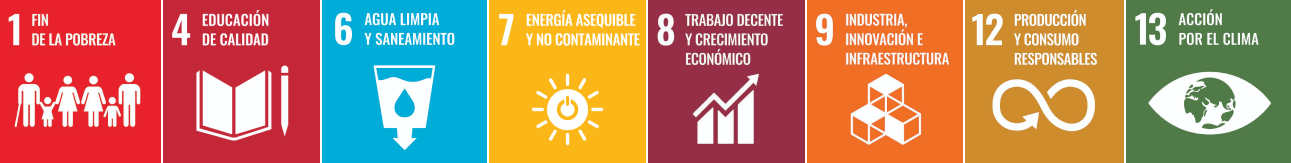
\includegraphics[width=\textwidth]{content/figures/ODS_TFG.png}
    \caption{Objetivos de Desarrollo Sostenible relacionados con este proyecto (\cite{ODS}).}
    \label{fig:ods_tfg}
  \end{figure}